\documentclass{beamer}
\usepackage[utf8]{inputenc}

\usetheme{Madrid}
\usecolortheme{default}
\usepackage{amsmath,amssymb,amsfonts,amsthm}
\usepackage{txfonts}
\usepackage{tkz-euclide}
\usepackage{listings}
\usepackage{adjustbox}
\usepackage{array}
\usepackage{tabularx}
\usepackage{gvv}
\usepackage{lmodern}
\usepackage{circuitikz}
\usepackage{tikz}
\usepackage{graphicx}
\usepackage{multicol}
\setbeamertemplate{page number in head/foot}[totalframenumber]

\usepackage{tcolorbox}
\tcbuselibrary{minted,breakable,xparse,skins}



\definecolor{bg}{gray}{0.95}
\DeclareTCBListing{mintedbox}{O{}m!O{}}{%
  breakable=true,
  listing engine=minted,
  listing only,
  minted language=#2,
  minted style=default,
  minted options={%
    linenos,
    gobble=0,
    breaklines=true,
    breakafter=,,
    fontsize=\small,
    numbersep=8pt,
    #1},
  boxsep=0pt,
  left skip=0pt,
  right skip=0pt,
  left=25pt,
  right=0pt,
  top=3pt,
  bottom=3pt,
  arc=5pt,
  leftrule=0pt,
  rightrule=0pt,
  bottomrule=2pt,

  colback=bg,
  colframe=orange!70,
  enhanced,
  overlay={%
    \begin{tcbclipinterior}
    \fill[orange!20!white] (frame.south west) rectangle ([xshift=20pt]frame.north west);
    \end{tcbclipinterior}},
  #3,
}
\lstset{
    language=C,
    basicstyle=\ttfamily\small,
    keywordstyle=\color{blue},
    stringstyle=\color{orange},
    commentstyle=\color{green!60!black},
    numbers=left,
    numberstyle=\tiny\color{gray},
    breaklines=true,
    showstringspaces=false,
}
%------------------------------------------------------------
%This block of code defines the information to appear in the
%Title page
\title %optional
{12.26}
\date{October  2025}
%\subtitle{A short story}

\author % (optional)
{BEERAM MADHURI - EE25BTECH11012}



\begin{document}


\frame{\titlepage}
\begin{frame}{Question}
Phani starts from point $\mathbf{P}$, goes North for $3$ km, and then East for $4$ km to reach point $\mathbf{Q}$. She then turns to face point $\mathbf{P}$ and goes $15$ km in that direction. She then goes North for $6$ km. How far is she from point $\mathbf{P}$, and in which direction should she go to reach point $\mathbf{P}$?

\begin{enumerate}
    \item[a)] $8$ km, East
    \item[b)] $12$ km, North
    \item[c)] $6$ km, East
    \item[d)] $10$ km, North
\end{enumerate}
\end{frame}
 
\begin{frame}{solution}
    \frametitle{finding the final position and direction of Phani:}
Let point $\mathbf{P}$  be the origin:
\begin{align}
\mathbf{P} = \begin{bmatrix} 0 \\ 0 \end{bmatrix}
\end{align}
Moving from  $\mathbf{P}$ to $\mathbf{Q}$\\
First, move North by 3 km:
\begin{align}
\mathbf{A} = \begin{bmatrix} 0 \\ 3 \end{bmatrix}
\end{align}
\end{frame}
\begin{frame}
Then, move East by 4 km:
\begin{align}
\mathbf{B} = \begin{bmatrix} 4 \\ 0 \end{bmatrix}
\end{align}

Position at point  $\mathbf{Q}$ is:
\begin{align}
\mathbf{Q} = \mathbf{P} + \mathbf{A} + \mathbf{B} \\= \begin{bmatrix} 0 \\ 0 \end{bmatrix} + \begin{bmatrix} 0 \\ 3 \end{bmatrix} + \begin{bmatrix} 4 \\ 0 \end{bmatrix} \\= \begin{bmatrix} 4 \\ 3 \end{bmatrix}
\end{align}
\end{frame}
\begin{frame}
Move 15 km Toward $\mathbf{P}$ from $\mathbf{Q}$\\
Direction vector from $\mathbf{Q}$ to $\mathbf{P}$:
\begin{align}
\mathbf{D} = \mathbf{P} - \mathbf{Q}\\
= \begin{bmatrix} 0 \\ 0 \end{bmatrix} - \begin{bmatrix} 4 \\ 3 \end{bmatrix} \\
= \begin{bmatrix} -4 \\ -3 \end{bmatrix}
\end{align}
\begin{align}
|\mathbf{D}| = \sqrt{(-4)^2 + (-3)^2}\\
= \sqrt{16 + 9} \\
= \sqrt{25} = 5
\end{align}
\end{frame}
\begin{frame}
\begin{align}
\hat{\mathbf{D}} = \frac{1}{5} \begin{bmatrix} -4 \\ -3 \end{bmatrix}
\end{align}
Now multiply by 15 km:
\begin{align}
\mathbf{C} = 15 \cdot \hat{\mathbf{D}}\\ = 3 \cdot \begin{bmatrix} -4 \\ -3 \end{bmatrix} \\
= \begin{bmatrix} -12 \\ -9 \end{bmatrix}
\end{align}
\end{frame}
\begin{frame}
New position :
\begin{align}
\mathbf{R} = \mathbf{Q} + \mathbf{C} \\
= \begin{bmatrix} 4 \\ 3 \end{bmatrix} + \begin{bmatrix} -12 \\ -9 \end{bmatrix} \\
= \begin{bmatrix} -8 \\ -6 \end{bmatrix}
\end{align}
Moving North by 6 km

\begin{align}
\mathbf{F} = \begin{bmatrix} 0 \\ 6 \end{bmatrix}
\end{align}
\end{frame}

\begin{frame}
Final position:
\begin{align}
\mathbf{S} = \mathbf{R} + \mathbf{F} \\
= \begin{bmatrix} -8 \\ -6 \end{bmatrix} + \begin{bmatrix} 0 \\ 6 \end{bmatrix} \\
=\begin{bmatrix} -8 \\ 0 \end{bmatrix}
\end{align}
Distance and Direction from Final Position to $\mathbf{P}$
\begin{align}
\mathbf{P} - \mathbf{S} \\
= \begin{bmatrix} 0 \\ 0 \end{bmatrix} - \begin{bmatrix} -8 \\ 0 \end{bmatrix} \\
= \begin{bmatrix} 8 \\ 0 \end{bmatrix}
\end{align}
\end{frame}
\begin{frame}
\textbf{Distance}:
\begin{align}
\|\mathbf{P} - \mathbf{S}\| = \sqrt{8^2 + 0^2} = 8 \text{ km}
\end{align}
\textbf{Direction}: Since the vector is along the positive x-axis, the direction is \textbf{East}.\\
$\therefore$ Option a is correct
\end{frame}

\begin{frame}[fragile]
\frametitle{Python Code}
\begin{lstlisting}
import matplotlib.pyplot as plt
# Define the points in the journey
p = (0, 0)
north_point = (0, 3)
q = (4, 3)
r = (-8, -6)
s = (-8, 0)
# Create the plot
plt.figure(figsize=(10, 8))
ax = plt.gca()
\end{lstlisting}
\end{frame}

\begin{frame}[fragile]
\frametitle{Python Code}
\begin{lstlisting}
# Plot the path segments
# 1. P to North Point
plt.plot([p[0], north_point[0]], [p[1], north_point[1]], 'r-o', label='Path 1: 3 km North')
plt.annotate('3 km', xy=(0.1, 1.5), xytext=(0.1, 1.5))
# 2. North Point to Q
plt.plot([north_point[0], q[0]], [north_point[1], q[1]], 'g-o', label='Path 2: 4 km East')
plt.annotate('4 km', xy=(2, 3.1), xytext=(2, 3.1))
\end{lstlisting}
\end{frame}

\begin{frame}[fragile]
\frametitle{Python Code}
\begin{lstlisting}
# 3. Q to R (towards P and beyond)
plt.plot([q[0], r[0]], [q[1], r[1]], 'b-o', label='Path 3: 15 km towards P')
# Add an arrow for this segment
ax.arrow(q[0], q[1], r[0]-q[0], r[1]-q[1], head_width=0.5, head_length=0.7, fc='blue', ec='blue', length_includes_head=True)
plt.annotate('15 km', xy=(-3, -2), xytext=(-3, -2), color='blue')
\end{lstlisting}
\end{frame}

\begin{frame}[fragile]
\frametitle{Python Code}
\begin{lstlisting}
# 4. R to S
plt.plot([r[0], s[0]], [r[1], s[1]], 'm-o', label='Path 4: 6 km North')
plt.annotate('6 km', xy=(-8.5, -3), xytext=(-8.5, -3), color='purple', rotation=90)

# 5. Final path from S to P
plt.plot([s[0], p[0]], [s[1], p[1]], 'k--o', label='Final: 8 km East to P')
\end{lstlisting}
\end{frame}

\begin{frame}[fragile]
\frametitle{Python Code}
\begin{lstlisting}
ax.arrow(s[0], s[1], p[0]-s[0], p[1]-s[1], head_width=0.5, head_length=0.7, fc='black', ec='black', length_includes_head=True)
plt.annotate('8 km', xy=(-4, 0.2), xytext=(-4, 0.2), color='black')
plt.text(p[0] - 0.5, p[1] - 0.5, 'P (Start)', fontsize=12)
plt.text(q[0] + 0.2, q[1] + 0.2, 'Q', fontsize=12)
plt.text(r[0] - 0.5, r[1] - 1, 'R', fontsize=12)
plt.text(s[0] - 1.5, s[1] + 0.2, 'S (Final)', fontsize=12)
\end{lstlisting}
\end{frame}

\begin{frame}[fragile]
\frametitle{Python Code}
\begin{lstlisting}
# Set plot limits and labels
plt.xlim(-15, 10)
plt.ylim(-10, 10)
plt.xlabel("East-West Direction (km)")
plt.ylabel("North-South Direction (km)")
plt.title("Phani's Journey")
plt.axhline(0, color='grey', lw=0.5)
plt.axvline(0, color='grey', lw=0.5)
plt.grid(True)
plt.gca().set_aspect('equal', adjustable='box')
plt.legend()
\end{lstlisting}
\end{frame}

\begin{frame}[fragile]
\frametitle{Python Code}
\begin{lstlisting}
# Add compass directions
plt.text(0, 9, 'North', ha='center', va='center', fontsize=10)
plt.text(0, -9, 'South', ha='center', va='center', fontsize=10)
plt.text(9, 0, 'East', ha='center', va='center', fontsize=10)
plt.text(-14, 0, 'West', ha='center', va='center', fontsize=10)

# Save the figure
plt.savefig("phanis_journey.png")
\end{lstlisting}
\end{frame}

\begin{frame}[fragile]
\frametitle{C Code}
\begin{lstlisting}
#include <stdio.h>
#include <math.h>

// A struct to represent a point with x and y coordinates
typedef struct {
    double x;
    double y;
} Point;
\end{lstlisting}
\end{frame}

\begin{frame}[fragile]
\frametitle{C Code}
\begin{lstlisting}
int main() {
    // Let the starting point P be the origin
    Point p = {0.0, 0.0};
    Point current_pos = {0.0, 0.0};

    printf("Simulating Phani's journey...\n");
    printf("Start at P: (%.1f, %.1f)\n", current_pos.x, current_pos.y);
\end{lstlisting}
\end{frame}

\begin{frame}[fragile]
\frametitle{C Code}
\begin{lstlisting}
    // 1. Goes North for 3 km
    current_pos.y += 3.0;
    printf("1. After moving North 3 km: (%.1f, %.1f)\n", current_pos.x, current_pos.y);

    // 2. Then East for 4 km to reach point Q
    current_pos.x += 4.0;
    Point q = current_pos;
    printf("2. After moving East 4 km to Q: (%.1f, %.1f)\n", current_pos.x, current_pos.y);
\end{lstlisting}
\end{frame}

\begin{frame}[fragile]
\frametitle{C Code}
\begin{lstlisting}
    // 3. Turns to face point P and goes 15 km
    // Vector from current position (Q) towards P
    double vec_to_p_x = p.x - q.x; // 0 - 4 = -4
    double vec_to_p_y = p.y - q.y; // 0 - 3 = -3

    // The distance between Q and P (magnitude of the vector)
    double dist_qp = sqrt(vec_to_p_x * vec_to_p_x + vec_to_p_y * vec_to_p_y);
\end{lstlisting}
\end{frame}

\begin{frame}[fragile]
\frametitle{C Code}
\begin{lstlisting}
    // Create a unit vector for the direction
    double unit_vec_x = vec_to_p_x / dist_qp;
    double unit_vec_y = vec_to_p_y / dist_qp;

    // Move 15 km along this direction
    current_pos.x += 15.0 * unit_vec_x;
    current_pos.y += 15.0 * unit_vec_y;
    printf("3. After moving 15 km towards P: (%.1f, %.1f)\n", current_pos.x, current_pos.y);
\end{lstlisting}
\end{frame}

\begin{frame}[fragile]
\frametitle{C Code}
\begin{lstlisting}
    // 4. Then goes North for 6 km
    current_pos.y += 6.0;
    printf("4. After moving North 6 km (Final Position): (%.1f, %.1f)\n\n", current_pos.x, current_pos.y);

    // Question 1: How far is she from point P?
    double final_distance = sqrt(pow(current_pos.x - p.x, 2) + pow(current_pos.y - p.y, 2));
\end{lstlisting}
\end{frame}

\begin{frame}[fragile]
\frametitle{C Code}
\begin{lstlisting}
    // Question 2: In which direction should she go to reach point P?
    // Vector from her final position back to P
    double dir_to_p_x = p.x - current_pos.x; // 0 - (-8) = 8

    printf("Final Answer:\n");
    printf("Distance from start point P: %.0f km\n", final_distance);
    printf("Direction to reach point P: ");
\end{lstlisting}
\end{frame}

\begin{frame}[fragile]
\frametitle{C Code}
\begin{lstlisting}
    if (dir_to_p_x > 0) {
        printf("East\n");
    } else if (dir_to_p_x < 0) {
        printf("West\n");
    } // simplified for this problem

    printf("This corresponds to option a) 8 km, East.\n");
    return 0;
}
\end{lstlisting}
\end{frame}

\begin{frame}[fragile]
\frametitle{Python and C Code}
\begin{lstlisting}
import ctypes
import math

# Define the Point struct using ctypes
class Point(ctypes.Structure):
    _fields_ = [("x", ctypes.c_double),
                ("y", ctypes.c_double)]
\end{lstlisting}
\end{frame}

\begin{frame}[fragile]
\frametitle{Python and C Code}
\begin{lstlisting}
def main():
    # Let the starting point P be the origin
    p = Point(0.0, 0.0)
    current_pos = Point(0.0, 0.0)

    print("Simulating Phani's journey...")
    print(f"Start at P: ({current_pos.x:.1f}, {current_pos.y:.1f})")
\end{lstlisting}
\end{frame}

\begin{frame}[fragile]
\frametitle{Python and C Code}
\begin{lstlisting}
    # 1. Goes North for 3 km
    current_pos.y += 3.0
    print(f"1. After moving North 3 km: ({current_pos.x:.1f}, {current_pos.y:.1f})")
    # 2. Then East for 4 km to reach point Q
    current_pos.x += 4.0
    q = Point(current_pos.x, current_pos.y)
    print(f"2. After moving East 4 km to Q: ({current_pos.x:.1f}, {current_pos.y:.1f})")
\end{lstlisting}
\end{frame}

\begin{frame}[fragile]
\frametitle{Python and C Code}
\begin{lstlisting}
    # 3. Turns to face point P and goes 15 km
    vec_to_p_x = p.x - q.x  # -4.0
    vec_to_p_y = p.y - q.y  # -3.0
    dist_qp = math.sqrt(vec_to_p_x**2 + vec_to_p_y**2)
    unit_vec_x = vec_to_p_x / dist_qp
    unit_vec_y = vec_to_p_y / dist_qp
\end{lstlisting}
\end{frame}

\begin{frame}[fragile]
\frametitle{Python and C Code}
\begin{lstlisting}
    current_pos.x += 15.0 * unit_vec_x
    current_pos.y += 15.0 * unit_vec_y
    print(f"3. After moving 15 km towards P: ({current_pos.x:.1f}, {current_pos.y:.1f})")
    # 4. Then goes North for 6 km
    current_pos.y += 6.0
    print(f"4. After moving North 6 km (Final Position): ({current_pos.x:.1f}, {current_pos.y:.1f})\n")
\end{lstlisting}
\end{frame}

\begin{frame}[fragile]
\frametitle{Python and C Code}
\begin{lstlisting}
    # Question 1: Distance from point P
    final_distance = math.sqrt((current_pos.x - p.x)**2 + (current_pos.y - p.y)**2)
    # Question 2: Direction to reach point P
    dir_to_p_x = p.x - current_pos.x
    print("Final Answer:")
    print(f"Distance from start point P: {final_distance:.0f} km")
\end{lstlisting}
\end{frame}

\begin{frame}[fragile]
\frametitle{Python and C Code}
\begin{lstlisting}
    if dir_to_p_x > 0:
        print("Direction to reach point P: East")
    elif dir_to_p_x < 0:
        print("Direction to reach point P: West")
    else:
        print("Direction to reach point P: Same line")
    print("This corresponds to option a) 8 km, East.")
if __name__ == "__main__":
    main()
\end{lstlisting}
\end{frame}
\begin{frame}
\begin{figure}
    \centering
    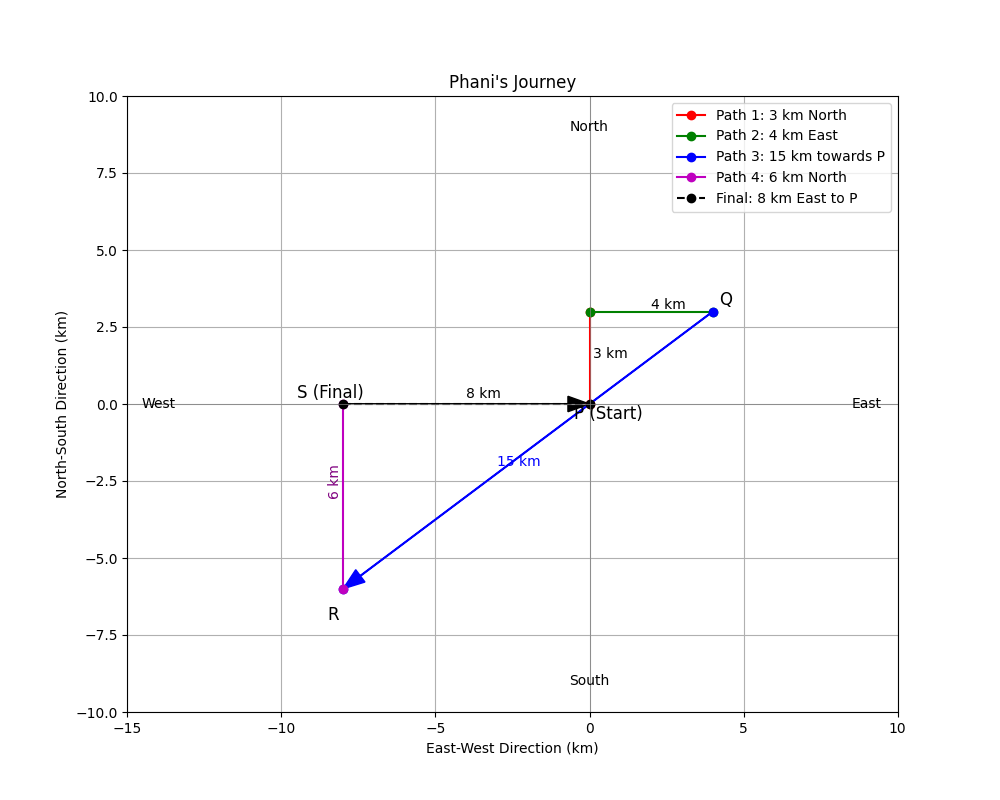
\includegraphics[width=0.75\columnwidth]{graph19.png}
    \caption{Plot}
    \label{fig:placeholder}
\end{figure}
\end{frame}

\end{document}